%%%%%%%%%%%%%%%%%%% Introduction %%%%%%%%%%%%%%%%%%%
The internet has opened many doors for humanity one of those being the apparent access to infinite information. Everyday people around the world generate over 400 million terabyte of new data \cite{matt2024}. This well of information has recently been adopted to train prominent artificial intelligence agents, like GPT-3 \cite{kashyap-2023}. Training these models even once is very expensive \cite{buchholz-2024} which makes it hard for developers to keep up with the seemingly unending flow of new data. Aside from this financial factor, the physical limitations of storage and computation time for all of these data files pose another problem for AI developers and demonstrates the need for selective model editing without retraining. On a smaller scale, AI often needs to adapt to more specialized use cases \cite{verwimp2024continuallearningapplicationsroad}. Pre-trained AI models, for example in smart watches, need to be able to adapt to their owner's habits in order to be fully functional.
Continual learning (CL), often referred to as lifelong learning or incremental learning, aims to solve ease these limitations for AI by dividing all available and future data into distinct sets, which are then processed sequentially \cite{verwimp2024continuallearningapplicationsroad}.

Training on distinct data sets, puts developers in front of a new problem: how can they make sure AI does not forget previously learned information? 

AI is built on artificial neural networks (ANN), a machine learning program, that makes decisions by mimicing a human brain \cite{ibm2025}. Although they are inspired by humans they currently lack the ability to look inward and reflect on themselves. Ergo, people need to find ways to determine what is important information for AI in order to enable efficient ways of "remembering". Understanding how ANNs make decisions is also important to build trust and confidence in AI \cite{Sudmann2020}. 

Their use cases go far beyond suggesting a new song for your playlist or correcting typos in a rushed text message. We have started to implement AI to drive cars or help with medical examinations. These tasks often come with variations, like driving in different weather conditions or recognizing more than one kind of tumor. It would be desirable to have a single AI that can learn these task when required and maybe even use previously learned information to help with the new training process. Like children first learn the alphabet and then use this knowledge to read and write texts, AI should leverage prior tasks to solve new ones.

Throughout this thesis I want to explore the possibilities and limitations of regularization as a CL method with some selected examples, as well as how advances in this field can contribute to a better understanding of ANNs. There have been thorough surveys on CL as a whole \cite{LW, verwimp2024continuallearningapplicationsroad, bidaki2025}, which provide a more complete overview of this field. This thesis separates itself from them by diving deeper into individual methodologies in order to demonstrate how regularization in CL has helped to extract importance measures in ANNs and which tasks can even be learned in such a setting.
Although continual learning is a general modeling concept, applicable in statistical inference as well as pattern driven prediction algorithms, it is mostly used in a machine learning context, more specifically in artificial neural networks (ANN). They are algorithms based on the functionality of a human brain and often designed for scenarios where data is seen in real-time, e.g. stock market predictions or power control systems. \citeauthor{Du_2019} \cite{Du_2019} and \citeauthor{Fahrmeir_2022} \cite{Fahrmeir_2022} provide an overview to this topic, which builds the foundation of this thesis. 

The simplest form of an ANN is a single linear classifier, called one-neuron perceptron, that devides a vector $x$ into two classes using a so-called activation function $h(\cdot)$. The neuron's input is given by
\begin{equation}
	\sum_{i = 1}^{n}{w_i x_i}+c = w^\top x+c
\end{equation}
where $n$ is the number of observations, $w$ a weight vector assigned to $x$ and $c$ the decision threshold. The two class regions are separated by the hyperplane%% \cite{Du_2019}
\begin{equation}
	w^\top x + c = 0
\end{equation}.
Using multiple neurons with the same activation function creates a one-layer perceptron and enables classification for more than two classes with the input
\begin{equation}
	\sum_{k = 1}^{m}\sum_{i=1}^{n}w_{k,i}x_i + c = (w_1^\top x + c, ..., w_m^\top x + c)^\top = W^\top x + c
\end{equation} 
, where $W$ is the $n\times m$ weight matrix and $m$ the number of classes. Given $h$ as the logistic function, a one-layer perceptron is equal to a multinomial logit model%%\cite{Fahrmeir_2022}
. Composing $l$ layers of neurons, Feed Forward NN (FFNN), allows for a more abstract representation of the data and finer class boundaries. Commonly, these layers are referred to as hidden layers, since only the input and output are observable. The unknown weight matrices $W_1, ..., W_l$ and the decision threshold $c$ are obtained by minimizing the empirical Risk of the network
\begin{equation}
	\mathcal{R}(f) = \sum_{i=1}^{n} L(f(x_i, \theta), y_i)
\end{equation}
, where $\theta$ are the unknown parameters and $L(\cdot)$ a loss function, which measures the discrepancy between the predicted values $\hat{y}_i = f(x_i, \theta)$ and the true values $y_i$. Risk minimization usually makes use of gradient-decent methods. They are numerical algorithms that converge to a local minimum in $\varepsilon$-neighborhood of the solution of parameters.
\begin{figure}[h!]
	\centering
	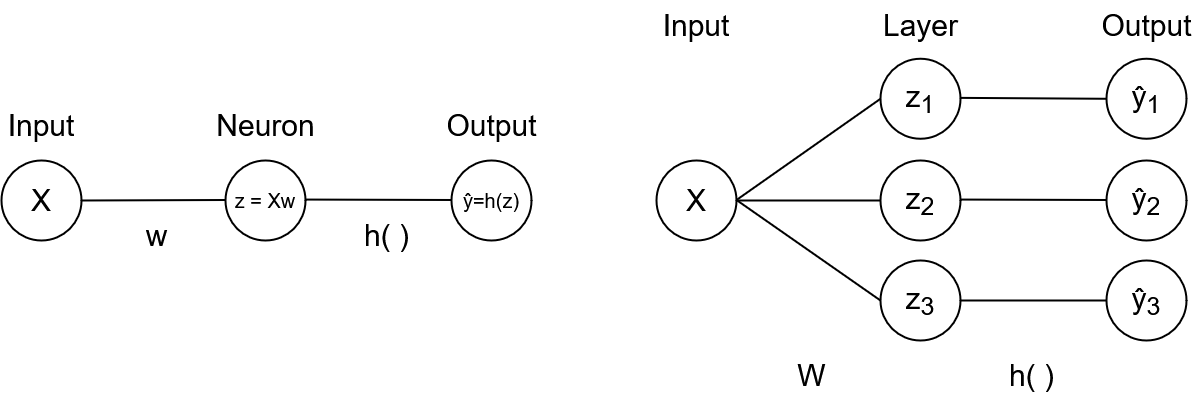
\includegraphics[width=0.9\textwidth]{img/perceptrons.png}
	\caption{A one-neuron perceptron (left) and a one-layer perceptron with 3 neurons (right).}
	\label{fig:P}
\end{figure}

In the following, modeling of a probability distribution over a data sample and learning how to predict the next output for an unseen data point will both be referred to as a \textit{task}. Both ideas are closely related, because inferred statistical models can be used to deduce long term behavior or to make a best guess about unobserved data.
%%%%%%%%%%%%%%%%%%% framework %%%%%%%%%%%%%%%%%%%
Throughout literature continual learning, in a statistical sense, means modeling a joint probability distribution, which is allowed to be infinitely expanded \cite{LW}. $T$ samples $D_t, t \in {1, ...,T}$ from different distributions $\mathbb{P}_t$ are processed sequentially. A single sample has the form $D_t = (X^{(t)},y^{(t)}) \in (\mathbb{R}^{n_t \times d_t}, \mathbb{R}^{n_t})$ with $X^{(t)}$ being the covariate matrix and $y^{(t)}$ the dependent variable. The $y^{(t)}|X^{(t)}$ are assumed to be conditionally independent but not necessarily identically distributed \cite{LW}. The joint distribution $\mathbb{P}^{(t)}$ of $Y^{(t)}|\mathcal{X}^{(t)} = \{y^{(i)}|X^{(i)}\}_{i=1}^t$ a model should have learned after seeing the $t$-th samples is then
\begin{equation}
	\mathbb{P}^{(t)}(Y^{(t)}|\mathcal{X}^{(t)}) = \prod_{i = 1}^{t}\mathbb{P}_i(y^{(i)}|X^{(i)})
\end{equation}
. Each tuple $(D_t, \mathbb{P}_t)$ may correspond to a distinct regression or classification task that is to be learned. The goal is to train a single model which is able to perform well on all tasks, although training happens sequentially and cannot necessarily revisit prior data samples. This systematic constraint implies that CL algorithms risk \textit{forgetting} previous tasks which will be explained in \autoref{cf}. For ease of notation, columns of a covariate matrix will be referred to as features and the dependent variable as label(s).
%%%%%%%%%%%%%%%%%%% Scenarios %%%%%%%%%%%%%%%%%%%
In regards to the label space \citeauthor{bidaki2025} \cite{bidaki2025} and \citeauthor{LW} \cite{LW} differentiate between eight CL scenarios:

\textit{Task-incremental learning} (TIL), \textit{Class-incremental learning} (CIL), \textit{Task-Free continual learning} (TFCL) and \textit{Online contiunal learning} (OCL) algorithms all aim to learn a distinct set of tasks, while providing a task identity, if not stated otherwise \cite{bidaki2025, LW}.
\begin{equation}
	y^{(i)} \cap y^{(i+1)} = \emptyset
\end{equation}

TIL allows task individual output layers or the training of separate models for each task. The challenge then is less about forgetting but finding a healthy balance between prediction accuracy and model complexity \cite{vandeVen2022}.

CIL restricts this approach by only training one model, which is introduced stepwise to different classification tasks. CIL only provides task identity during training \cite{vandeVen2022}. For example, with samples $t$ an agent learns to classify hats or gloves and with sample $t+1$ shirts or pants. When testing, it is then also required to classify hats or shirts.

TFCL does not provide any task identity to the model and only focuses on labels \cite{aljundi2019tfcl}.

OCL limits its sample sizes to one and focuses on real-time training \cite{bidaki2025, LW}.

\textit{Domain-incremental learning} (DIL) algorithms seek to learn multiple tasks that share the same label space [\citenum{bidaki2025}]. For example, first learning to drive during sunny weather and later while it is rainy. One could view this as a version of task-incremental learning, where task identity is secondary as all tasks have the same data labels. Thus, design based strategies to inhibit forgetting are not possible \cite{vandeVen2022}.
\begin{equation}
	y^{(i)}=y^{(i+1)} \nRightarrow \mathbb{P}(y^{(i)}) = \mathbb{P}(y^{(i+1)})
\end{equation}

\textit{Instance-incremental learning} (IIL) algorithms learn one common task for all training samples \cite{bidaki2025, LW}.
This is a special case of DIL where a model learns the distribution of one "domain" while only ever accessing snippets of the total available data. For example, each sample contains new real-world photographs of cats to classify. Assuming OCL only learns one task, OCL is a special case of IIL where each data point is seen in sequence.
\begin{equation}
	y^{(i)}=y^{(i+1)}, \mathbb{P}(y^{(i+1)}) = \mathbb{P}(y^{(i+1)}) \Rightarrow \mathbb{P}(Y^{(t)})=\mathbb{P}(y^{(i)})
\end{equation}

\textit{Blurred Boundary continual learning} (BBCL), in contrast to all others so far, allows partially overlapping label spaces \cite{bidaki2025,LW}.

\textit{Continual Pre-training} (CPT) aims to improve knowledge transfer with sequentially arriving pre-training data \cite{bidaki2025, LW}.

As presented, CL can occur in various environments. The connecting problem is memorizing an old task without blocking out new ones and vice versa. In particular, after each training step, the neural network needs to update its weight parameters in a way that the new weights can describe the relationship between all $(y^{(i)}, X^{(i)})$ pairs.
%%%%%%%%%%%%%%%%%%% Stability-Plasticity Trade-off %%%%%%%%%%%%%%%%%%%
The challenge of continual learning is to strike a balance between stability and plasticity. Models should retain knowledge of past tasks: stability, while being flexible enough to incorporate information from new data: plasticity. The sequential training nature of CL changes the weights acquired form learning task A to accommodate for a new task B. This abrupt loss of information is called catastrophic forgetting \cite{FRENCH1999128, Mcclelland1995, MCCLOSKEY1989109, Ratcliff1990ConnectionistMO}. A naive approach to solving this dilemma would be storing and replaying data to the network with each training step. This is impractical because the amount of data needed to be stored is proportional to the number of tasks learned.

\citeauthor{evron2022} \cite{evron2022} define forgetting as
\begin{equation}
	F(t) = 1/t \sum_{i=1}^{t}\lVert X^{(i)} w^{(t)} - y^{(i)} \rVert^2
\end{equation}
They have analyzed catastrophic forgetting in linear regression under the assumptions that values of $X$ are bounded by 1, tasks are jointly realizable with a bounded (by 1) norm, and there are more parameters than observations in each sample. Realizability assumes the existence of true model weights s.t. $y^{(t)}=X^{(t)}w^*$ \cite{Shalev-Shwartz}. This enables them to focus only on minimizing the distance between new and old model weights. In their work they find an upper bound for forgetting
\begin{equation}
	\sup F(t) = \sup 1/t \sum_{i=1}^{t}\lVert(I-Q_i)Q_t ... Q_1\rVert^2
\end{equation}
where $Q_i$ are the projections onto the solution spaces of $w^{(i)}$, 

i.e. $Q_i := I - X^{(i)\top}(X^{(i)} X^{(i)\top})^{-1} X^{(i)}$.

So far many methods of minimizing catastrophic forgetting have been developed. Their core ideas can be summarized to \textit{Replay} methods \cite{chaudhry2019,rebuffi2017icarlincrementalclassifierrepresentation, aljundi2019gradientbasedsampleselection}, \textit{Optimization} methods \cite{lopezpaz2022gradientepisodicmemorycontinual, javed2019metalearningrepresentationscontinuallearning, mirzadeh2020understandingroletrainingregimes}, \textit{Architecual} methods \cite{mallya2018piggybackadaptingsinglenetwork, ebrahimi2020adversarialcontinuallearning, fernando2017pathnetevolutionchannelsgradient} and \textit{Regularization} methods, which will be discussed in \autoref{reg0}.

In order to evaluate how well these methods work \citeauthor{lopezpaz2022gradientepisodicmemorycontinual} \cite{lopezpaz2022gradientepisodicmemorycontinual} suggest three performance metrics which measure how well a model can use learned tasks to solve new ones and how much knowledge of old tasks needs to be "unlearend" / forgotten to learn new ones.
%%%%%%%%%%%%%%%%%%% Metrics %%%%%%%%%%%%%%%%%%%
In the following each sample $D_t = (X^{(t)}, y^{(t)})$ is divided into a training split $D_t^{(train)} = (X^{(t)}_{(train)}, y^{(t)}_{(train)})$ and a testing split $D_t^{(test)} = (X^{(t)}_{(test)}, y^{(t)}_{(test)})$. The chosen splitting method is arbitrary. The training process for each sample will be conducted with $D_t^{(train)}$ and evaluation with $D_t^{(test)}$.

\citeauthor{lopezpaz2022gradientepisodicmemorycontinual} \cite{lopezpaz2022gradientepisodicmemorycontinual} come up with three different measures for model predictability, stability and plasticity. I will focus on their dynamic forms given by \citeauthor{díazrodríguez2018dontforgetforgettingnew} \cite{díazrodríguez2018dontforgetforgettingnew}, because they have been adapted for in training use, i.e. they represent a model's current state after the $t$-th training step.

\textit{Accuracy} $\mathbf{A}$ represents a models performance i.e. how well the predictions $\hat{y}^{(t)}_{(test)}$ align with the true values of $y^{(t)}_{(test)}$ for a metric $\mu$ . When $A_{i,k} = \mu(\hat{y}_{(test)}^{(k)}, y_{(test)}^{(k)}) \in [0,1]$ is the accuracy measured on the $k$-th test split after the $i$-th training step, then
\begin{equation}
	\mathbf{A} = \frac{2}{t(t-1)}\sum_{i \geq k }^{t} A_{i,k}
\end{equation}
is the average accuracy after the $t$-th training step over all test splits $D_k^{(test)}, k <= t$.

\textit{Backward Transfer} $\mathbf{BWT}$ evaluates a models stability. The metric quantifies the influence that learning sample $D_{t+1}^{(train)}$ has on the performance over test sample $D_t^{(test)}$ \cite{lopezpaz2022gradientepisodicmemorycontinual}. Given the above mentioned individual \textit{Accuracy} scores $A_{i,k}$
\begin{equation}
	\mathbf{BWT} = \frac{2}{t(t-1)} \sum_{i=2}^{t}\sum_{k=1}^{i-1}(A_{i,k}-A_{k,k})
\end{equation}
is the average backward transfer after the $t$-th training step. Note that $\mathbf{BWT}$ can be negative. This property captures (catastrophic) forgetting \cite{LW}.

\textit{Forward Transfer} $\mathbf{FWT}$ is a metric for model plasticity. Complementary to BWT, \textit{Forward Transfer} measures how previous training steps influence the current one. Again, the individual \textit{Accuracy} scores are the basis for this evaluation metric. The average influence of old training steps on the model performance after the $t$-th step is:
\begin{equation}
	\mathbf{FWT} = \frac{2}{t(t-1)}\sum_{i < k }^{t} A_{i,k}
\end{equation}.

One of the motivations for CL is limited memory space for data which is why storing a test sample for each task is limiting in the long run when the number of tasks goes to infinity. A metric that directly measures the relationship between stability and plasticity on the model is presented by \citeauthor{mirzadeh2020understandingroletrainingregimes}\cite{mirzadeh2020understandingroletrainingregimes}. They use the maximum eigenvalue of the loss' Hessian $\lambda^{max}$ to describe the width of their approximation of the loss' minimum. They hypothesize that the \textit{wideness} of this minimum correlates with the forgetting rate of the respective model.

Given $W^{(t)*}$ and $W^{(t+1)*}$, the optimal parameters after learning the $t$-th and $(t+1)$-th task and $L_t(\cdot)$ and $L_{t+1}(\cdot)$ the corresponding loss function, \citeauthor{mirzadeh2020understandingroletrainingregimes} formulate the upper bound
\begin{equation}\label{2TA}
	F_t = L_t(W^{(t+1)*}) - L_t(W^{(t)*}) \approx \frac{1}{2}{\Delta W}^\top \nabla^2 L_t(W^{(t)*}) \Delta W \leq \frac{1}{2}\lambda_t^{max}\lVert \Delta W \rVert^2
\end{equation}
for the forgetting $F_t$ of the $t$-th task. They approximate $L_t(W^{(t+1)*})$ around $W^{(t)*}$ with a second order Taylor approximation, where $\nabla^2$ is the Hessian for $L_t$ and $\Delta W$ the difference between $W^{(t+1)*}$ and $W^{(t)*}$. They argue that the loss can be approximated this way, because of its almost convex path around the minimum, for models that have more observations per sample than parameters.

Furthermore, ${\Delta W}$ is dependent on the training process of the $(t+1)$-th task, which depends on the random sample it is trained on, so one can view the differences in parameters as a random vector that follows some distribution parameterized by the eigenvalues of $\nabla^2 L_t(W^{(t)*})$ \cite{mirzadeh2020understandingroletrainingregimes}. Controlling the distance between old and new weights, as well as $\lambda^{max}$ of subsequent tasks seems to be the key to mitigating forgetting \cite{mirzadeh2020understandingroletrainingregimes}.

%%%%%%%%%%%%%%%%%%% Figure 2 %%%%%%%%%%%%%%%%%%%
\usetikzlibrary{datavisualization.formats.functions}
\begin{figure}[h!]
	\centering
	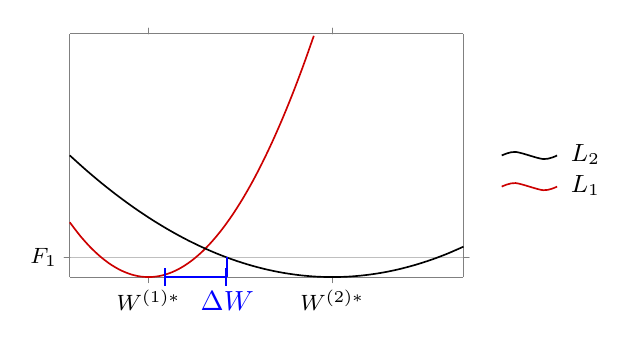
\begin{tikzpicture}[baseline]
		\datavisualization [
		scientific axes, 
		x axis = {ticks={major at={-0.2 as $W^{(1)*}$, 0.5 as $W^{(2)*}$}}},
		y axis = {max value = 0.2, ticks and grid ={major at={0.016 as $F_1$}}},
		visualize as smooth line/.list={w1,w2},
		style sheet=strong colors,
		w1 = {label in legend = {text=$L_2$}},
		w2 = {label in legend = {text=$L_1$}},
		data/format=function
		]
		data [set=w1] {
			var x : interval [-0.5:1];
			func y = 0.1 * (\value x - 0.5) * (\value x - 0.5);
		}
		data [set=w2] {
			var x : interval [-0.5:0.43];
			func y = 0.5 * (\value x  + 0.2) * (\value x + 0.2);
		};
		\usetikzlibrary{arrows.meta}
		\draw [thick, blue, |-|] (1.2, 0) -- (2, 0);
		\draw [thick, blue] (2, 0) -- (2, 0.25);
		\draw [blue] (2, -0.3) node {$\Delta W$};
	\end{tikzpicture}
	\caption{Depending on the curvature of $L_1$ and $L_2$, different $\Delta w$ result in different forgetting rates.}
	\label{fig:02}
\end{figure}
%%%%%%%%%%%%%%%%%%% Regularization %%%%%%%%%%%%%%%%%%%
As mentioned in \autoref{cf}, one way to address the stability-plasticity problem is the use of regularization. This approach adds a penalty term to the loss function of a model. Usually this penalty term depends on the model parameters. Later we will also see some methods that directly penalize the output of a model. I will begin by categorizing the regularization methods that I have found through out my research and present some selected examples. After this overview of current possibilities in regularization techniques, I will present approaches at unifying and generalizing them.

In \cite{evron2022,li2024fixeddesignanalysisregularizationbased} the authors introduce a rudimentary approach to regularization in CL, called \textit{ordinary conitunal learning}. It is used as a worst case comparison for their contribution to this field and is the basis for the upper bound on forgetting in \autoref{cf}.

Despite its limitations, I believe that it is beneficial to start this section with ordinary CL. In the beginning I will reduce the complexity of continual learning to two subsequent linear regression problems, which simplifies the entry into the field.

Ordinary continual learning \cite{evron2022,li2024fixeddesignanalysisregularizationbased, zhao2024statisticaltheoryregularizationbasedcontinual} assumes a CL problem with $T=2$ linear regression models $y^{(t)} = X^{(t)}w^* + \epsilon_t, \epsilon_t \sim N(0, \sigma^2), t \in \{1,2\}$, the task corresponding samples $D_t = (X^{(t)}, y^{(t)}) \in (\mathbb{R}^{n_t \times d}, \mathbb{R}^{n_t})$ and a covariance matrix of $\hat{w}^{(t)}$, $\Sigma_t = 1/n^{(t)} X^{(t)\top} X^{(t)}$. To estimate the first task parameters $\hat{w}^{(1)}$, ordinary continual learning algorithm performs an ordinary least square minimization over the first sample set $D_1$, i.e. $\hat{w}^{(1)} = (X^{(1)\top}X^{(1)})^{-1}X^{(1)\top} y^{(1)}$. In the second training sequence, ordinary continual learning fits $w^{(2)}$ to the residuals of task one with respect to $X^{(2)}$. The new parameters $\hat{w}^{(2)}$ are then:
\begin{equation}
	\hat{w}^{(2)} = \hat{w}^{(1)} + (X^{(2)\top}X^{(2)})^{-1}X^{(2)\top} (y^{(2)} - X^{(2)}\hat{w}^{(1)})
\end{equation}
In their analysis of ordinary continual learning,\citeauthor{zhao2024statisticaltheoryregularizationbasedcontinual} \cite{zhao2024statisticaltheoryregularizationbasedcontinual} show that it suffers from constant forgetting and provide the lower bound for its forgetting:
\begin{equation}
	F_t = \mathbb{E}(\lVert \hat{w}^{(t)} - w^* \rVert_2^2) \geq \frac{\sigma^2}{\lambda_{max}^{(t)}}
\end{equation}
where $\lambda_{max}^{(t)}$ maximum eigenvalue of $\Sigma_t$.

Since the inverse of the negative Hessian of the neg-log likelihood of $\hat{w}^{(t)}$ is an estimator for $\Sigma_t$, ordinary CL a good example for the "worst case" of CL. Neither the maximum eigenvalue of nor the distance between old and new parameters are controlled, thus forgetting happens constantly. Ergo methodologies that control at least one of them are required.
%%%%%%%%%%%%%%%%%%% Regularization via Parameters %%%%%%%%%%%%%%%%%%%
%%%%%%%%%%%%%%%%%%% L2 Norm %%%%%%%%%%%%%%%%%%%
%% L2 Continual Ridge Regression %% 
Expanding on the naive \textit{ordinary continual learning} approach, \citeauthor{li2024fixeddesignanalysisregularizationbased} \cite{li2024fixeddesignanalysisregularizationbased} suggest an adaptation of the Ridge penalty for continual learning, dubbed \textit{continual ridge regression} (CRR) \cite{li2024fixeddesignanalysisregularizationbased, zhao2024statisticaltheoryregularizationbasedcontinual}. For estimating $w^{(2)}$, they introduce a Ridge-like penalty term
\begin{equation}\label{ridge}
	\pen_{R}(w) = \lambda\lVert w - \hat{w}^{(1)}\rVert_2^2
\end{equation}
which centers the new weights around the previously estimated $\hat{w}^{(1)}$ instead of 0. Instead of using penalized least squares, the authors decide to perform a penalized mean squared error regression. %% change to MSE in Reg0 chapter
\begin{equation}
	\begin{split}
		\hat{w}^{(2)} &= \arg\min_{w} \frac{1}{n}\lVert y^{(2)} - X^{(2)}w\rVert_2^2 + \pen(w) \\
		&= (X^{(2)\top} X^{(2)}+\lambda n I)^{-1}(X^{(2)\top} y^{(2)} +\lambda n \hat{w}^{(1)})
	\end{split}
\end{equation}
Unlike regular ridge regression, CRR is unbiased. The proofs for an unbiased CRR can be found in Appendix \ref{crr}. \citeauthor{li2024fixeddesignanalysisregularizationbased} acknowledge that centering around $\hat{w}^{(1)}$ enables a more stable learning environment, compared to ordinary CL, but still struggles when tasks are too dissimilar. Another reason CRR has difficulties learning dissimilar tasks, is that all dimensions of $w$ are penalized equally throughout all tasks, i.e.
\begin{equation}\label{ridgeMat}
	\pen_R(w) = (w - \hat{w}^{(1)})^\top \lambda I (w - \hat{w}^{(1)})
\end{equation} . When learning a joint probability distribution, as in DIL, the information contained in $D_t$ about $w$ can vary across coordinates.
%% Generalized L2 %%
As a solution to this, \citeauthor{zhao2024statisticaltheoryregularizationbasedcontinual} \cite{zhao2024statisticaltheoryregularizationbasedcontinual} propose a generalized quadratic penalty for linear regression tasks, which allows individual regularization strengths in all directions of $w$. 

From now on I will no longer restrict Cl to only two tasks.

\textit{Generalized l2-regression} (GR) \cite{zhao2024statisticaltheoryregularizationbasedcontinual} extends CRR and ordinary CL. It is asymptotically equivalent to an unrestricted model, i.e. a model that can access all data samples at the same time. \citeauthor{zhao2024statisticaltheoryregularizationbasedcontinual} define the unrestricted estimation error $\mathcal{L}(\cdot)$ over all tasks as:
\begin{equation}\label{oracle}
	\mathcal{L}(\hat{w}^{(T)}) = \sum_{i}^{d} \frac{\sigma^2}{\alpha^{(1)}_i n^{(^)}+ ... + \alpha^{(T)}_i n^{(^T)}}
\end{equation}
with $\alpha^{(t)}_i$ being the $i$-th eigenvector of $\Sigma_t$. Note that this error is monotonously decreasing as $T$ gets bigger, thus no forgetting \cite{zhao2024statisticaltheoryregularizationbasedcontinual}. GRs goal is to find a matrix $\Lambda^{(t)}$ for \eqref{ridgeMat}, which properly accommodates a samples contribution to each $\hat{w}_i$ so that the combined estimation error of $L(\hat{w}^{(t)})$ converges to $\mathcal{L}(\hat{w}^{(T)})$. The authors are able to prove that for $\Lambda^{(t)}$, a diagonizable matrix with $\Lambda^{(t)} = U \Delta U^\top, \Delta = \diag(\delta_1, ... \delta_d)$, the loss $L(\hat{w}^{(t)})$ is bounded by $\mathcal{L}(\hat{w}^{(T)})$ if the diagonal values of $\Delta$ are 
\begin{equation}
	\delta_i = \frac{\sigma^2 / (U_i^\top w^*)^2 + \alpha^{(1)}_i n^{(1)} + ... + \alpha^{(t-1)}_i n^{(t-1)}}{n^{(t)}}
\end{equation}
For large $n^{(t)}$, $\frac{\sigma^2 / (U_i^\top w^*)^2}{n^{(t)}}$ becomes small enough to be neglected and \cite{zhao2024statisticaltheoryregularizationbasedcontinual} approximate $\tilde{\Lambda}^{(t)} = \frac{1}{n^{(t)}}\sum_{i = 1}^{t-1} n^{(i)}\Sigma_i$.

In this linear setting, the $\Sigma_i$ are equivalent to the Hessian and Fisher information matrix of the loss function. This means that every change$w_i$ is penalized proportionally to the information sample $D_t$ contains about its previous state.

\citeauthor{zhao2024statisticaltheoryregularizationbasedcontinual} \cite{zhao2024statisticaltheoryregularizationbasedcontinual} demonstrate how powerful regularization can be. However, that all tasks share the individual solution $w^*$ is not always realistic. \citeauthor{JK} \cite{JK} tackle this problem by taking a Bayesian look at the joint distribution over all tasks.

%% EWC %% 
One of the most influential regularization approaches for CL is the \textit{elastic weight consolidation} penalty (EWC) by \citeauthor{JK} \cite{zhao2024statisticaltheoryregularizationbasedcontinual, zenke2017continuallearningsynapticintelligence, Husz_r_2018, li2024fixeddesignanalysisregularizationbased, titsias2020functionalregularisationcontinuallearning, yin2021optimizationgeneralizationregularizationbasedcontinual, loo2020generalizedvariationalcontinuallearning, benzing2021unifyingregularisationmethodscontinual}. They suggest measuring weight importance via the Fisher information matrix. Kirkpatrick et al. justify this approach through a probabilistic view of neural networks. They no longer want to find the parameters that best fit the data pattern, but find the most probable model weights, depending on a given data sample. Using Bayes' Rule and the assumption of independent samples, they express the conditional probability $\mathbb{P}(w|\mathcal{D}^{(t)}), \mathcal{D}^{(t)} = \{D_1, ..., D_t\}$ of the weights as \footnote{\citeauthor{JK} \cite{JK} only provide equation \eqref{ewcBayes} for 2 tasks. The expansion for $t$ tasks ,which is used here, can be found in Appendix \ref{ewcB}.}
\begin{equation}\label{ewcBayes}
	\log\mathbb{P}(w|\mathcal{D}^{(t)}) = \log\mathbb{P}(D_{t}|w) + \log\mathbb{P}(w|\mathcal{D}^{(t-1)}) - \log\mathbb{P}(D_t)
\end{equation}
and point out that all of the information about all prior tasks is in $\mathbb{P}(w|\mathcal{D}^{(t-1)})$, but is unavailable due to the sequential training constraint. To overcome this problem, the authors approximate the missing posterior as a Gaussian with expected value $\hat{w}^{(t-1)}$ and precision matrix $F = diag(\sum_{i < t}\mathcal{I}_i(w_1), ..., \sum_{i < t }\mathcal{I}_i(w_d))$ where $\mathcal{I}_i(w_j), j \in \{1, ..., d\}$ are the Fisher information of $w_i$ from the $i$-th training step, thus $\mathbb{P}(w|\mathcal{D}^{(t-1)}) \dot{\sim} N(\hat{w}^{(t-1)}, F^{-1})$. The resulting penalty function is a weighted Ridge penalty, where the squared deviation from the previous parameters is weighed against its Fisher information:
\begin{equation}\label{EWC}
	\pen_{EWC}(w) = \frac{\lambda}{2}(w - \hat{w}^{(t-1)})^\top F (w - \hat{w}^{(t-1)})
\end{equation}
Note that if the loss is chosen as the negative log-likelihood, EWC is equal to the 2nd Taylor approximation of a generalized forgetting rate in \eqref{2TA}. In this case the Fisher information matrix is equivalent to the Hessian of the loss. In general the EWC penalty encourages gradient decent to follow along trajectories of $w_i$ with low Fisher information which are thus less prone to forgetting.

%% SI %%
\citeauthor{zenke2017continuallearningsynapticintelligence} \cite{zenke2017continuallearningsynapticintelligence} argue that a static estimate of parameter importance between training steps is not enough and suggest a dynamic solution, \textit{synaptic intelligence} (SI), along the loss' gradient. Similar to EWC, GR and CRR they impose a quadratic penalty on the loss:
\begin{equation}\label{SI}
	\pen_{SI}(w) = \frac{\lambda}{2} (w - \hat{w}^{(1)})^\top H (w - \hat{w}^{(1)})
\end{equation}
where $H$ is the diagonal of the Hessian of the current loss $L(X^{(2)}, y^{(2)}, w)$.

%% MAS %%
The next example is the \textit{memory aware synapses} (MAS) penalty \cite{aljundi2018memoryawaresynapseslearning}. Similar to EWC and SI it focuses on task disjoint CL. To further improve the idea of gradient based importance, the authors consider the model output $h(\cdot)$ and measure its sensitivity to changes in the model parameters. The importance matrix $\Omega$ holds the mean gradients over all samples of the squared L2-normed outputs i.e. $\Omega^{(t)} = 1/n \sum_{i \leq n} \nabla \lVert h(x^{(t)}_i, \hat{w}^{(t)}) \rVert_2^2$. With the resulting penalty function:
\begin{equation}\label{MAS}
	\pen_{MAS}(w)=\lambda (w - \hat{w}^{(t-1)})^\top \Omega^{(t-1)} (w - \hat{w}^{(t-1)})
\end{equation}
\citeauthor{aljundi2018memoryawaresynapseslearning} \cite{aljundi2018memoryawaresynapseslearning} aim to provide a flexible importance measure, which can be calculated on any representative data set, since it does not depend on the model loss.

Generally regularization in CL, with a squared penalty, restricts large deviations from the previously estimated parameters if these $w_i^{(t-1)}$ were important to prior learnings. Given some importance matrix $A$, the generalized squared-l2 penalty for the next training step is:
\begin{equation}\label{l2pen}
	pen_{l2}(w) = \lambda (w - \hat{w}^{(t)})^\top A (w - \hat{w}^{(t)})
\end{equation}
Although FIM and Hessian at large are not identical, \citeauthor{benzing2021unifyingregularisationmethodscontinual} \cite{benzing2021unifyingregularisationmethodscontinual} demonstrate how SI and MAS are still linked to FIM. \citeauthor{yin2021optimizationgeneralizationregularizationbasedcontinual} \cite{yin2021optimizationgeneralizationregularizationbasedcontinual} provide a unifying analysis of squared penalties in CL. They conclude that the difference between the true loss over all tasks and its approximation depends on two factors: first a sample effect, which is negligible for increasing $n^{(t)}$, and second the technical error of the approximation. Thus they encourage more accurate approximations. Furthermore, \citeauthor{liu2018rotatenetworksbetterweight} \cite{liu2018rotatenetworksbetterweight} point out that the diagonal approximation of the Fisher information matrix has potential to lead gradient decent "off-path" and use rotations of the parameter space to adjust.

%%%%%%%%%%%%%%%%%%% Regularization via Parameters %%%%%%%%%%%%%%%%%%%
%%%%%%%%%%%%%%%%%%% L1 Norm %%%%%%%%%%%%%%%%%%%
The Ridge-like penalties provide control over a model's stability. Because their approximations become increasingly inaccurate with each new training step, they encourage smaller steps away from the current state of the model as training continues \cite{yin2021optimizationgeneralizationregularizationbasedcontinual}. All of the algorithms presented so far imply that all parameters are, to some degree, useful across all tasks. \textit{Adaptive Group Sparsity based Continual Learning} (AGS-CL) \cite{jung2021continuallearningnodeimportancebased} and the \textit{Dynamically Expandable Network} algorithm (DEN) \cite{yoon2018lifelonglearningdynamicallyexpandable} question this and suggest a Grouped-LASSO penalty. The parameter groups are determined by the neurons they connect to or come from. This way the model can benefit from already established weights and simultaneously use free neurons to fit task specific parameters.

%% AGGS_CL %%
AGS-CL argues that a selective use of network nodes could be beneficial when dealing with unrelated tasks. Their idea is to influence model plasticity via Grouped-LASSO regularization. Similar to the already seen penalties, the AGS-CL algorithm makes use of an importance matrix $\Omega\in\mathbb{R}^{l\times \nu}$ to decide whether weights connecting to a node should be protected or not.
\begin{equation}
	\Omega^{(t)} = \Omega^{(t-1)} + \sum_{j=1}^{l}\sum_{k=1}^{\nu} \left[\frac{1}{n^{(t)}}\sum_{i=1}^{n^{(t)}}\relu_{j,k}(x_i^{(t)})\right]
\end{equation}
With $\relu_{j,k}(x) = \max(0, x)$ as the activation function of node $k$ in layer $j$, the task specific penalty term is then:
\begin{equation}\label{agscl}
	\begin{split}
		\pen_{AGSCL}(W)= &\mu\sum_{j,k \leq l,\nu} \id(\Omega_{j,k}^{(t-1)} = 0)\lVert W_{j,k} \rVert_2 \\
		&+ \lambda \sum_{j,k \leq l,\nu} \id(\Omega_{j,k}^{(t-1)} > 0)\lVert W_{j,k} - \hat{W}_{j,k}^{(t-1)}\rVert_2
	\end{split}
\end{equation}
All nodes with importance 0 are penalized directly and thus their weights might get estimated to 0. Deviations from very important nodes, i.e. nodes with high $\Omega$-value, can be prevented completely due to the second penalty term.

Note that AGS-CL relies on a fixed network structure. With increasing task number, the ability "to freeze" entire nodes could potentially stop learning all together, if new tasks are too unrelated to prior knowledge. For example, a classifier with $t$ output nodes needs to learn $t+1$ categories. 

%% DEN %%
DEN acknowledges this problem \cite{yoon2018lifelonglearningdynamicallyexpandable}. In order to provide a higher degree of plasticity, DEN identifies the task related sub-networks of the model and retrains it to evaluate if additional nodes are required to adequately adjust to the new data. To identify which established network parameters are useful to the new task, DEN uses a standard LASSO penalty on the weights directly connecting to the output layer. In case the sub-network's loss is too high, DEN gradually expands each layer with additional nodes, which are again selected via grouped-LASSO. The final network is then again estimated via Ridge-regularization as in \eqref{ridge}. 

Overall DEN aims to keep a sparse network for individual tasks through the abuse of prior knowledge and simultaneously is able to adapt to unrelated tasks by expanding its network structure when needed. This relates DEN closely to methods that directly influence a network's structure and hints that the targeted combination of CL algorithms could balance out individual weaknesses. 

Another way of controlling changes in a model arises when looking at its outputs. Such methods generally use some representation of the old model to guide the new learning process. Since CL has clear training stages, these approaches can be seen as offline knowledge distillation \cite{Gou_2021}, where the previous model acts like a teacher to the current one.
%%%%%%%%%%%%%%%%%%% Regularization of Function Space %%%%%%%%%%%%%%%%%%%
%% LwF %%
\citeauthor{li2017learningforgetting} \cite{li2017learningforgetting} provide with \textit{Learning without Forgetting} (LwF) one of the earliest advances in this field. LwF assumes (multi-) image-classification tasks and specifies a logistic loss function $L(y, h(x)) = -y \log h(x)$ and the softmax activation function $h(x) = \exp(x_i)/\sum_{i\leq \#classes}\exp(x_i)$ in the output layer. In detail, LwF makes a prediction $y_o^{(t)}$, based on the old model, for the new sample before the next training cycle. These predictions are then used to penalize the fitted values $\hat{y}_o^{(t)}$ from the new model:
\begin{equation}\label{LwF}
	\pen_{LwF}(W) = \lambda \sum_{i = 1}^{\#classes}-y_{o,i}^{(t)} \log \hat{y}_{o,i}^{(t)}
\end{equation}
Considering the predefined loss above, then $\pen_{LwF}$ could be viewed as a 2nd parallel learner. It is important to note that $\hat{y}_o^{(t)}$ and $y_o^{(t)}$ are not the actual values but some weighted version of themselves, in order to help the new network to better approximate old outputs (Knowledge Distillation loss \cite{hinton2015distillingknowledgeneuralnetwork}). LwF also makes some structural adjustments with each training step by adding a number of fully connected neurons to the output layer if the new sample contains unseen class labels. Without this, the network would force predictions in the same label space for all tasks and thus not be able to adjust to the expanding multinomial distribution of $\mathbb{P}(Y^{(t)}) = \prod_{i = 1}^{t}\mathbb{P}(y^{(i)})$.

%% DRI %%
Instead of relying on an estimate of the previous true fitted values $\hat{y}^{(1)}, ..., \hat{y}^{(t-1)}$, \citeauthor{Wang_Liu_Duan_Tao_2022} \cite{Wang_Liu_Duan_Tao_2022} suggest with \textit{Deep Retrieval and Imagination} (DRI) storing a small sample $M$ of all previous tasks. In their work, they also focus on image classification with known labels (CIL or DIL). To ensure that $M$ is representative of all $t-1 + 1$ tasks, the authors use a resampling strategy inspired by \citeauthor{welling_2009} \cite{welling_2009} when adding new data points to it. During training DRI does not only aim to learn the combined sample $D^{(t)} \cup M$ but also just $M$. The additional penalty terms center new model outputs of already seen tasks around their previous fittings, which are calculated on a copy of the old model.
\begin{equation}\label{dri}
	\begin{split}
		\hat{W}^{(t)} = &\arg\min_{W} L(W, D^{(t)} \cup M)\\
		&+ \beta L(W, M) + \frac{\alpha}{n^{(M)}}\sum_{i}^{n^{(M)}}\lVert f(W, x_i^{(M)}) - f(W^{(t-1)}, x_i^{(M)}) \rVert_2^2
	\end{split}
\end{equation}
In their work \citeauthor{Wang_Liu_Duan_Tao_2022} come to a very similar conclusion, as \citeauthor{yin2021optimizationgeneralizationregularizationbasedcontinual} \cite{yin2021optimizationgeneralizationregularizationbasedcontinual} in their analysis of generalized l2 penalties in CL. The discrepancy between the true joint training error and their surrogate loss consists yet again of an approximation error and a finite-sample effect. They alleviate the approximation error by padding $M$ with generated data from itself.

%% FRCL %%
\setlength{\parindent}{20pt}
As a final example for function space regularization, I want to present the \textit{functional regularization for continual learing} (FRCL) algorithm by \citeauthor{titsias2020functionalregularisationcontinuallearning} \cite{titsias2020functionalregularisationcontinuallearning}. They take a Bayesian perspective on NN, such that the model outputs $\hat{y}^{(t)}$ are a random vector depending on the output function $f^{(t)}(\cdot)$. In contrast to prior Bayesian approaches to CL, FRCL only focuses on the outermost parameter layer, connecting to the output, and optimizes everything else: $f^{(t)}(x^{(t)}) = w^{(t)\top} g(x^{(t)}; \theta)$ where $g(x;\theta)$ is the composition of all hidden layers and their parameters $\theta$. In each training step, they approximate the task specific output distributions $\mathbb{P}(y^{(i)})$ with a Gaussian Process (GP) \cite{Ludkovski2025} $p(y^{(t)}|f^{(t)}(X^{(t)}))$ and store a small collection of its inducing points $\tilde{D}_t=(\tilde{X}^{(t)}, \tilde{y}^{(t)} = f^{(t)}(\tilde{X}^{(t)})\in \mathbb{R}^{d\times m^{(t)}}\times \mathbb{R}^{m^{(t)}} $. These inducing points are found via minimizing the Kullback-Leibler divergence KL from their approximated distribution to the true GP. The base line model then minimizes 
\begin{equation}\label{bFrcl}
	L^{(t)}(\theta, w) = L_t(D^{(t)}, w^{(t)}, \theta) + \sum_{i=1}^{t-1}\frac{n^{(i)}}{m^{(i)}}  L_i(\tilde{D}_i,w^{(i)}, \theta)
\end{equation}
where each $L_i$ is a task specific loss and $m^{(i)}$ the size of the inducing sample of task $i$.
This approach makes a couple of assumptions and approximations about different parts of the network, which will be summarized in the remaining part of this subsection, as well as a non-trivial transformation to get to the explicit loss function.

\setlength{\parindent}{0pt}
\citeauthor{titsias2020functionalregularisationcontinuallearning} begin by assuming a normal prior on the outer-layer parameters $p_\theta(w^{(t)}) = N(0, \sigma^2_wI)$ with its variational approximation $q(w^{(t)}) = N(w^{(t)}|\mu_{w^{(t)}}, \Sigma_{w^{(t)}})$, as well as a linear kernel \cite{Ludkovski2025} $K_{X^{(t)}} = \sigma_w^2g(X^{(t)};\theta)^\top g(X^{(t)};\theta)$ for the network. Where $\mu_{w^{(t)}} \in \mathbb{R}^t$ and $\Sigma_{w^{(t)}} = C_{w^{(t)}}C_{w^{(t)}}^\top$ with $C_{w^{(t)}}$ is a square lower triangular matrix with positive diagonal elements. With this, the general posterior distribution over all function values is
\begin{equation}
	p(y^{(t)}|f^{(t)}(X^{(t)})) = \int p\left(y^{(t)}|w^{(t)\top} g(x^{(t)};\theta)\right)q(w^{(t)}) dw^{(t)}
\end{equation}
The authors acknowledge that regularization could already happen with this expression of the posterior. They argue that it would be a very expensive process and make use of the above mentioned approximation via inducing points $\tilde{D}_t$ to reduce the required storage space per task. These points are learned by minimizing the Kullback-Leibler divergence KL from $q(w^{(t)})$ to $p_\theta(w^{(t)})$. Now the task specific loss $L_t$ becomes the evidence lower bound (ELBO) \cite{Blei_2017} for $D_t$ and is maximized over $\theta$ and $q(w^{(t)})$. The authors transform the ELBO to the following equation, referencing multiple other papers. For convenience $w^{(t)\top} g(x^{(t)};\theta)$ will be referred to as $f^{(t)}$ further on.
\begin{equation}\label{elbo}
	L_t(\theta, q(w^{(t)})) = \sum_{i=1}^{n^{(t)}} \mathbb{E}_{q(w^{(t)})}\left[\log p(y_i^{(t)}|f_i^{(t)})\right] - \kl\left(q(w^{(t)})\Vert p_\theta(w^{(t)})\right)
\end{equation}
After this set up, we can focus on summarizing the last step, finding the penalty term for FRCL. Considering the learned inducing points $\tilde{D}_t$ and the joint distribution \(p(y^{(t)}, f^{(t)},\allowbreak \tilde{y}^{(t)})\), the true posterior can now be written as 
\begin{equation}
	p(y^{(t)}|f^{(t)}) = p_\theta(f^{(t)}|\tilde{y}^{(t)}, y^{(t)})p_\theta(\tilde{y}^{(t)}|y^{(t)})
\end{equation}

which can now be approximated by the GP $p_\theta(f^{(t)}| \tilde{y}^{(t)})q(\tilde{y}^{(t)})$, with $p_\theta(f^{(t)}|\tilde{y}^{(t)}) = N(f^{(t)}|\mu_{f^{(t)}},\allowbreak \Sigma_{f^{(t)}})$ and $q(\tilde{y}^{(t)}) = N(\tilde{y}^{(t)}|\mu_{\tilde{y}^{(t)}}, C_{\tilde{y}^{(t)}}C_{\tilde{y}^{(t)}}^\top)$, only depending on the variational distribution over $\tilde{y}^{(t)}$. Thus FRCL needs new task samples to be able to explain the approximated posteriors $q(\tilde{y}^{(t)})$ of every prior tasks so far seen. This leads to the penalty term:
\begin{equation}\label{penElbo}
	\pen_{FRCL}(\theta, q(w^{(t)})) = - \sum_{j=1}^{t-1}\kl(q(\tilde{y}^{(j)})\Vert p_\theta(\tilde{y}^{(j)}))
\end{equation}
with $p_\theta(\tilde{y}^{(t)}) = N(\tilde{y}^{(t)}|0, K_{\tilde{X}^{(t)}})$. Recalling that $\tilde{y}^{(t)}$ still depends on the distribution over $w^{(t)}$, its distributional parameters are $\mu_{\tilde{y}^{(t)}} = g(\tilde{X}^{(t)}; \theta)^\top \mu_{w^{(t)}}$ and $C_{\tilde{y}^{(t)}} = g(\tilde{X}^{(t)}; \theta)^\top C_{w^{(t)}}$. Ultimately, the algorithm stores $(\tilde{X}^{(t)}, \mu_{\tilde{y}^{(t)}}, C_{\tilde{y}^{(t)}})$ to memorize task $t$ for future training cycles.

As we have seen, FRCL mitigates forgetting via saving an approximate posterior of the current task's probability distribution and regularizes coming tasks through a KL penalty term. The authors acknowledge that their approach has similarities to replay-based methods, further strengthening the assumption that a combination of different methods could be the key to successful CL.
%%%%%%%%%%%%%%%%%%% Note on evaluation %%%%%%%%%%%%%%%%%%%
At last it is important to note that this thesis does not provide information about the compared performance of each of the presented regularization techniques. Despite the fact that all authors have conducted their own experiments, a formal comparison, through survey work alone, is not possible at the moment. Each research team has used different data sets and the overlap of used reference models is very small. Additionally, ordinary CL, CRR and GR serve a strictly theoretical purpose, since their assumptions strongly restrict their real world applications. The teams behind them have only provided experimental proof of concepts via simulated data and acknowledge their limitations.

Nevertheless, the conducted experiments highlight the influence of EWC on the field. It is used as a reference model for the majority of the presented regularization methods \cite{zenke2017continuallearningsynapticintelligence, aljundi2018memoryawaresynapseslearning, yoon2018lifelonglearningdynamicallyexpandable, jung2021continuallearningnodeimportancebased, titsias2020functionalregularisationcontinuallearning}.

Another point worth highlighting is that MINST and CIFAR are the most used data bases for the showcased methodologies \cite{zenke2017continuallearningsynapticintelligence,yoon2018lifelonglearningdynamicallyexpandable, jung2021continuallearningnodeimportancebased, Wang_Liu_Duan_Tao_2022}. This raises the question if their overuse biases research towards a race for the "best fit".
%%%%%%%%%%%%%%%%%%% Conclusion %%%%%%%%%%%%%%%%%%%
As we have seen regularization on parameters is a powerful tool to stabilize a continual learning algorithm. Stability is a desirable quality when tasks are similar but can lead to a learning collapse if they are not. Direct regularization of parameters could lead to unwanted generalization problems for future tasks, thus slowing down the rate at which new tasks can be learned. These shortcomings could be alleviated by using the outputs for parameter estimation. Penalizing deviations in the output might lead to an overall more flexible learner. Such approaches require extra memory to store information about past tasks. This drawback can be mitigated by effective sampling to min-max memory size and retained information or incorporating a second generative model. Efforts on balancing stability and model plasticity have also been made with sparse penalties, which aim to reduce individual network connection or even entire nodes to 0. They reduce the task specific complexity of the model in order to achieve better generalization across all tasks. Requiring tasks which can be generalized well in the first place which explains why the linear task assumption is so widespread.
Yet in order to learn a distinct set of tasks, like in CIL, shared label spaces seem too restrictive for one fixed network. Therefore, some allow for an expansion of the network to accommodate for new task specific requirements, such as a larger output space or general model plasticity.
Overall the advantages and flaws of regularization in CL demonstrate the two fundamental criteria \cite{LW} for successful CL, intra- and inter-task generalizability.